
%% bare_conf.tex
%% V1.4b
%% 2015/08/26
%% by Michael Shell
%% See:
%% http://www.michaelshell.org/
%% for current contact information.
%%
%% This is a skeleton file demonstrating the use of IEEEtran.cls
%% (requires IEEEtran.cls version 1.8b or later) with an IEEE
%% conference paper.
%%
%% Support sites:
%% http://www.michaelshell.org/tex/ieeetran/
%% http://www.ctan.org/pkg/ieeetran
%% and
%% http://www.ieee.org/


% *** Authors should verify (and, if needed, correct) their LaTeX system  ***
% *** with the testflow diagnostic prior to trusting their LaTeX platform ***
% *** with production work. The IEEE's font choices and paper sizes can   ***
% *** trigger bugs that do not appear when using other class files.       ***                          ***
% The testflow support page is at:
% http://www.michaelshell.org/tex/testflow/



\documentclass[10pt, conference, letterpaper]{IEEEtran}
% Some Computer Society conferences also require the compsoc mode option,
% but others use the standard conference format.
%
% If IEEEtran.cls has not been installed into the LaTeX system files,
% manually specify the path to it like:
% \documentclass[conference]{../sty/IEEEtran}





% Some very useful LaTeX packages include:
% (uncomment the ones you want to load)


% *** MISC UTILITY PACKAGES ***
%
%\usepackage{ifpdf}
% Heiko Oberdiek's ifpdf.sty is very useful if you need conditional
% compilation based on whether the output is pdf or dvi.
% usage:
% \ifpdf
%   % pdf code
% \else
%   % dvi code
% \fi
% The latest version of ifpdf.sty can be obtained from:
% http://www.ctan.org/pkg/ifpdf
% Also, note that IEEEtran.cls V1.7 and later provides a builtin
% \ifCLASSINFOpdf conditional that works the same way.
% When switching from latex to pdflatex and vice-versa, the compiler may
% have to be run twice to clear warning/error messages.






% *** CITATION PACKAGES ***
%
%\usepackage{cite}
% cite.sty was written by Donald Arseneau
% V1.6 and later of IEEEtran pre-defines the format of the cite.sty package
% \cite{} output to follow that of the IEEE. Loading the cite package will
% result in citation numbers being automatically sorted and properly
% "compressed/ranged". e.g., [1], [9], [2], [7], [5], [6] without using
% cite.sty will become [1], [2], [5]--[7], [9] using cite.sty. cite.sty's
% \cite will automatically add leading space, if needed. Use cite.sty's
% noadjust option (cite.sty V3.8 and later) if you want to turn this off
% such as if a citation ever needs to be enclosed in parenthesis.
% cite.sty is already installed on most LaTeX systems. Be sure and use
% version 5.0 (2009-03-20) and later if using hyperref.sty.
% The latest version can be obtained at:
% http://www.ctan.org/pkg/cite
% The documentation is contained in the cite.sty file itself.






% *** GRAPHICS RELATED PACKAGES ***
%
\ifCLASSINFOpdf
  % \usepackage[pdftex]{graphicx}
  % declare the path(s) where your graphic files are
  % \graphicspath{{../pdf/}{../jpeg/}}
  % and their extensions so you won't have to specify these with
  % every instance of \includegraphics
  % \DeclareGraphicsExtensions{.pdf,.jpeg,.png}
\else
  % or other class option (dvipsone, dvipdf, if not using dvips). graphicx
  % will default to the driver specified in the system graphics.cfg if no
  % driver is specified.
  % \usepackage[dvips]{graphicx}
  % declare the path(s) where your graphic files are
  % \graphicspath{{../eps/}}
  % and their extensions so you won't have to specify these with
  % every instance of \includegraphics
  % \DeclareGraphicsExtensions{.eps}
\fi
% graphicx was written by David Carlisle and Sebastian Rahtz. It is
% required if you want graphics, photos, etc. graphicx.sty is already
% installed on most LaTeX systems. The latest version and documentation
% can be obtained at: 
% http://www.ctan.org/pkg/graphicx
% Another good source of documentation is "Using Imported Graphics in
% LaTeX2e" by Keith Reckdahl which can be found at:
% http://www.ctan.org/pkg/epslatex
%
% latex, and pdflatex in dvi mode, support graphics in encapsulated
% postscript (.eps) format. pdflatex in pdf mode supports graphics
% in .pdf, .jpeg, .png and .mps (metapost) formats. Users should ensure
% that all non-photo figures use a vector format (.eps, .pdf, .mps) and
% not a bitmapped formats (.jpeg, .png). The IEEE frowns on bitmapped formats
% which can result in "jaggedy"/blurry rendering of lines and letters as
% well as large increases in file sizes.
%
% You can find documentation about the pdfTeX application at:
% http://www.tug.org/applications/pdftex





% *** MATH PACKAGES ***
%
%\usepackage{amsmath}
% A popular package from the American Mathematical Society that provides
% many useful and powerful commands for dealing with mathematics.
%
% Note that the amsmath package sets \interdisplaylinepenalty to 10000
% thus preventing page breaks from occurring within multiline equations. Use:
%\interdisplaylinepenalty=2500
% after loading amsmath to restore such page breaks as IEEEtran.cls normally
% does. amsmath.sty is already installed on most LaTeX systems. The latest
% version and documentation can be obtained at:
% http://www.ctan.org/pkg/amsmath





% *** SPECIALIZED LIST PACKAGES ***
%
%\usepackage{algorithmic}
% algorithmic.sty was written by Peter Williams and Rogerio Brito.
% This package provides an algorithmic environment fo describing algorithms.
% You can use the algorithmic environment in-text or within a figure
% environment to provide for a floating algorithm. Do NOT use the algorithm
% floating environment provided by algorithm.sty (by the same authors) or
% algorithm2e.sty (by Christophe Fiorio) as the IEEE does not use dedicated
% algorithm float types and packages that provide these will not provide
% correct IEEE style captions. The latest version and documentation of
% algorithmic.sty can be obtained at:
% http://www.ctan.org/pkg/algorithms
% Also of interest may be the (relatively newer and more customizable)
% algorithmicx.sty package by Szasz Janos:
% http://www.ctan.org/pkg/algorithmicx




% *** ALIGNMENT PACKAGES ***
%
%\usepackage{array}
% Frank Mittelbach's and David Carlisle's array.sty patches and improves
% the standard LaTeX2e array and tabular environments to provide better
% appearance and additional user controls. As the default LaTeX2e table
% generation code is lacking to the point of almost being broken with
% respect to the quality of the end results, all users are strongly
% advised to use an enhanced (at the very least that provided by array.sty)
% set of table tools. array.sty is already installed on most systems. The
% latest version and documentation can be obtained at:
% http://www.ctan.org/pkg/array


% IEEEtran contains the IEEEeqnarray family of commands that can be used to
% generate multiline equations as well as matrices, tables, etc., of high
% quality.




% *** SUBFIGURE PACKAGES ***
%\ifCLASSOPTIONcompsoc
%  \usepackage[caption=false,font=normalsize,labelfont=sf,textfont=sf]{subfig}
%\else
%  \usepackage[caption=false,font=footnotesize]{subfig}
%\fi
% subfig.sty, written by Steven Douglas Cochran, is the modern replacement
% for subfigure.sty, the latter of which is no longer maintained and is
% incompatible with some LaTeX packages including fixltx2e. However,
% subfig.sty requires and automatically loads Axel Sommerfeldt's caption.sty
% which will override IEEEtran.cls' handling of captions and this will result
% in non-IEEE style figure/table captions. To prevent this problem, be sure
% and invoke subfig.sty's "caption=false" package option (available since
% subfig.sty version 1.3, 2005/06/28) as this is will preserve IEEEtran.cls
% handling of captions.
% Note that the Computer Society format requires a larger sans serif font
% than the serif footnote size font used in traditional IEEE formatting
% and thus the need to invoke different subfig.sty package options depending
% on whether compsoc mode has been enabled.
%
% The latest version and documentation of subfig.sty can be obtained at:
% http://www.ctan.org/pkg/subfig




% *** FLOAT PACKAGES ***
%
%\usepackage{fixltx2e}
% fixltx2e, the successor to the earlier fix2col.sty, was written by
% Frank Mittelbach and David Carlisle. This package corrects a few problems
% in the LaTeX2e kernel, the most notable of which is that in current
% LaTeX2e releases, the ordering of single and double column floats is not
% guaranteed to be preserved. Thus, an unpatched LaTeX2e can allow a
% single column figure to be placed prior to an earlier double column
% figure.
% Be aware that LaTeX2e kernels dated 2015 and later have fixltx2e.sty's
% corrections already built into the system in which case a warning will
% be issued if an attempt is made to load fixltx2e.sty as it is no longer
% needed.
% The latest version and documentation can be found at:
% http://www.ctan.org/pkg/fixltx2e


%\usepackage{stfloats}
% stfloats.sty was written by Sigitas Tolusis. This package gives LaTeX2e
% the ability to do double column floats at the bottom of the page as well
% as the top. (e.g., "\begin{figure*}[!b]" is not normally possible in
% LaTeX2e). It also provides a command:
%\fnbelowfloat
% to enable the placement of footnotes below bottom floats (the standard
% LaTeX2e kernel puts them above bottom floats). This is an invasive package
% which rewrites many portions of the LaTeX2e float routines. It may not work
% with other packages that modify the LaTeX2e float routines. The latest
% version and documentation can be obtained at:
% http://www.ctan.org/pkg/stfloats
% Do not use the stfloats baselinefloat ability as the IEEE does not allow
% \baselineskip to stretch. Authors submitting work to the IEEE should note
% that the IEEE rarely uses double column equations and that authors should try
% to avoid such use. Do not be tempted to use the cuted.sty or midfloat.sty
% packages (also by Sigitas Tolusis) as the IEEE does not format its papers in
% such ways.
% Do not attempt to use stfloats with fixltx2e as they are incompatible.
% Instead, use Morten Hogholm'a dblfloatfix which combines the features
% of both fixltx2e and stfloats:
%
% \usepackage{dblfloatfix}
% The latest version can be found at:
% http://www.ctan.org/pkg/dblfloatfix




% *** PDF, URL AND HYPERLINK PACKAGES ***
%
%\usepackage{url}
% url.sty was written by Donald Arseneau. It provides better support for
% handling and breaking URLs. url.sty is already installed on most LaTeX
% systems. The latest version and documentation can be obtained at:
% http://www.ctan.org/pkg/url
% Basically, \url{my_url_here}.




% *** Do not adjust lengths that control margins, column widths, etc. ***
% *** Do not use packages that alter fonts (such as pslatex).         ***
% There should be no need to do such things with IEEEtran.cls V1.6 and later.
% (Unless specifically asked to do so by the journal or conference you plan
% to submit to, of course. )


% correct bad hyphenation here
\hyphenation{op-tical net-works semi-conduc-tor}

\usepackage{color}
\usepackage{amsthm}
\usepackage{amsmath}
\usepackage{subfigure}
\usepackage{graphicx} 

\usepackage{setspace}

\usepackage{algorithm}
\usepackage{algpseudocode}
\usepackage{tabularx,ragged2e,booktabs,caption}

\newtheorem{mydef}{Definition}
\newtheorem{mylma}{Lemma}

\newcommand\eg{{\em e.g.}}
\newcommand\ie{{\em i.e.}}
\newcommand\bigo{{\mathcal{O}}}
\newcommand{\hz}[1]{\textcolor{red}{[hz: #1]}}

\begin{document}
%
% paper title
% Titles are generally capitalized except for words such as a, an, and, as,
% at, but, by, for, in, nor, of, on, or, the, to and up, which are usually
% not capitalized unless they are the first or last word of the title.
% Linebreaks \\ can be used within to get better formatting as desired.
% Do not put math or special symbols in the title.
\title{Hummingbird: A Novel Approach of Finding the Optimal Configuration for Big Data Analytics}


% author names and affiliations
% use a multiple column layout for up to three different
% affiliations
\author{Paper ID: 1570388224
% Y. Richard Yang$^{*+}$ \\
% Tongji University$^*$ \hspace{0.5cm}
% Yale University$^+$
}

% \author{\IEEEauthorblockN{Haizhou Du}
% \IEEEauthorblockA{School of Electrical and\\Computer Engineering\\
% Georgia Institute of Technology\\
% Atlanta, China  30332--0250\\
% Email: http://www.michaelshell.org/contact.html}
% \and
% \IEEEauthorblockN{Homer Simpson}
% \IEEEauthorblockA{Twentieth Century Fox\\
% Springfield, USA\\
% Email: homer@thesimpsons.com}
% \and
% \IEEEauthorblockN{James Kirk\\ and Montgomery Scott}
% \IEEEauthorblockA{Starfleet Academy\\
% San Francisco, California 96678--2391\\
% Telephone: (800) 555--1212\\
% Fax: (888) 555--1212}}

% conference papers do not typically use \thanks and this command
% is locked out in conference mode. If really needed, such as for
% the acknowledgment of grants, issue a \IEEEoverridecommandlockouts
% after \documentclass

% for over three affiliations, or if they all won't fit within the width
% of the page, use this alternative format:
% 
%\author{\IEEEauthorblockN{Michael Shell\IEEEauthorrefmark{1},
%Homer Simpson\IEEEauthorrefmark{2},
%James Kirk\IEEEauthorrefmark{3}, 
%Montgomery Scott\IEEEauthorrefmark{3} and
%Eldon Tyrell\IEEEauthorrefmark{4}}
%\IEEEauthorblockA{\IEEEauthorrefmark{1}School of Electrical and Computer Engineering\\
%Georgia Institute of Technology,
%Atlanta, Georgia 30332--0250\\ Email: see http://www.michaelshell.org/contact.html}
%\IEEEauthorblockA{\IEEEauthorrefmark{2}Twentieth Century Fox, Springfield, USA\\
%Email: homer@thesimpsons.com}
%\IEEEauthorblockA{\IEEEauthorrefmark{3}Starfleet Academy, San Francisco, California 96678-2391\\
%Telephone: (800) 555--1212, Fax: (888) 555--1212}
%\IEEEauthorblockA{\IEEEauthorrefmark{4}Tyrell Inc., 123 Replicant Street, Los Angeles, California 90210--4321}}




% use for special paper notices
%\IEEEspecialpapernotice{(Invited Paper)}




% make the title area
\maketitle

% As a general rule, do not put math, special symbols or citations
% in the abstract
% \begin{abstract}
% \end{abstract}
\begin{abstract}
Real time and cost-effective analytics for “Big Data” is now a key ingredient for success in many businesses, scientific research and engineering disciplines, and government endeavors. The Apache Spark platform—which consists of an extensible MapReduce execution engine, pluggable resilient distributed storage engines, and a range of procedural to declarative interfaces—is a mainstream choice for big data analytics. Unfortunately, most beginner of big data analytics—like software engineer, computational scientists, systems researchers, and business analysts—lack the expertise to configure the big data analytics system setting to get good performance. Due to each of them has hundreds of parameters for tunning. However, it is challenging to automatically identify the best configuration for a diversity of applications. In generally, Spark’s performance out of the box leaves much to be desired, leading to suboptimal use of resources, time, and money (in pay as-you-go clouds platform, like AWS, Azure etc.). We introduce Hummingbird: a novel approach of finding optimal configuration for big data analytics. It builds on Spark while adapting to user needs and system workloads to provide good performance, help users to understand and manipulate the many tuning knobs in Spark. Furthermore, experimental results show the Hummingbird can get the best configuration considering the running time and computational efficiency. Finally, the experimental results also show that the performance can get average 28\% gain with the Hummingbird compared with the default configuration of Spark. Certainly, Hummingbird can also be applied on other mainstream big data analytics systems.

\end{abstract}

\IEEEpeerreviewmaketitle


\section{introduction}
\par With the rapid and continuous development of big data analyze like distributed natural language processing \cite{brants2007large}, deep learning for image recognition \cite{dean2012Large}, genome analysis \cite{L2010cloudcomputing}, astronomy \cite{Berriman2010application} and particle accelerator data processing \cite{bird2011}. These applications differ from traditional analytics workloads (e.g., SQL queries) in that they are not only data-intensive but also computation-intensive, and typically run for a long time (and hence are expensive). Along with new workloads, we have seen widespread adoption of efficient big data anaytics platform with large datasets being hosted \cite{commoncrawlurl}, and the emergence of sophisticated analytics services, such as machine learning, being offered by data anaytics providers\cite{Machinelearningurl}.

\par According to IDC(Internet Data Center) predictions by 2020, the size of the digital universe will exceed 44ZB \cite{IDC2012}. So that we have entering the era of big data, and big data analytics technologies have attracted more and more attention from the academia, industry and governments in recent years. The traditional computing model in the era of big data cannot meet the demands of performance and efficiency, Hadoop \cite{apachehadoop}, Spark \cite{apachespark}, Storm \cite{apachestorm} and other distributed frameworks emerge as time goes on. Among several big data frameworks, Apache Spark has become the most popular and universal big data processing platform because of its excellent performance and rich application scenarios support.

\par With the wide application of Spark, it also exposes some problems in practical applications. One of the most important aspects is the performance problem. Due to unreasonable parameter configuration of Spark, the performance of Spark applications is difficult to achieve theoretical peak speed of computer, so how to optimize the performance of Spark applications is one problem that is worthy of research.

\par Apache Spark has more than 180 configuration parameters, which can be adjusted by users according to their own specific application so as to optimize the performance \cite{apachespark}. This is the most simple and effective way to optimize the performance of Spark applications. On the one hand, a lots of parameters enable a lot of opportunities for significant performance improvement by careful parameter tuning, but on the other hand, the large parameter space and the complex interactions among the parameters make the appropriate parameter tuning a challenging task.

\par New practitoners of big data analytics like computational scientists and systems researchers lack the experitse to tune Spark to get good performance. Currently, there are two ways to tuning the configuration parameters of Spark platforms. Firstly, these parameters are tuned manually by trial and error, which is ineffective and time consuming due to a lots of parameters and the complex interactions among the parameters. In order to overcome the disadvantages of tuning parameters manually, some researchers proposed a cost-based (analytical) performance modeling method to tuning the parameters of Hadoop platform \cite{apachehadoop}. However, Spark is much different from Hadoop in the underlying implementation mechanism, so that we can not use this method on Spark directly. Meanwhile, it suffers from several weakness when modeling Spark platform based on cost. First, cost-based modeling is a white box approach where a deep and wide knowledge about a system’s internals is required, and since the system that comprises the software stack (operating system, JVM, Spark, and workloads) and the hardware stack is very complex, it becomes very hard to capture this complexity with the cost-based model. Secondly, Spark has several customizable components where users can plug in their own policies, such as scheduling and encryption policies, which makes it necessary for the performance model to support these different policies.

\par These drawbacks motivate us to explore new approach based performance models, which are black box models. Compared with the existing approaches, black box models have two main advantages. First, the recommendations of an Automatic tuning using these models are based on observations of the actual system performance with logging information. Second, they are usually more simple to build as there is no need for detailed information about the system’s internals. Therefore, our proposed method relies on optimization theory to build the performance model, which makes it more robust and flexible.

\par The rest of the paper is organized as follows. The related work is discussed in Section \ref{sec:related}. A brief overview of Apache Spark and some definition are presented in Section \ref{sec:definition}. A performance model for multiple model fusion based on machine learning and optimization method of spark platform will be proposed in Section \ref{sec:approach}. Experimental methodology and experimental result analysis are given in Section \ref{sec:evaluation}. Finally, the conclusions and future work are summarized in Section \ref{sec:conclusion}. As a appendix, All of our selected parameters which are most important to the optimal configuration of Spark are listed in the Section \ref{sec:appendix} .

\section{Related Work}\label{sec:related}
\par Performance optimization of big data System has been one of the hot research areas in recent years due to the wide adoption of big data analytic platforms. But most of research works are based on the MapReduce computing framework or Hadoop platform. Starfish [5] uses cost-based modeling and simulation to search the desired job configurations for MapReduce workloads. AROMA [6] automates job configuration and resource allocation through leveraging a two phase machine learning and optimization framework for heterogeneous clouds. In reference [7], the authors point out that Hadoop's scheduler can cause severe performance
degradation in heterogeneous environments and present a new scheduler called Longest Approximate Time to End. Another work [8] focused on analyzing the variant effect of resource consumption of different settings for the Map and Reduce slots. In reference [9], the authors address these problems by presenting the Profiling and Performance Analysis-based System (PPABS) framework, which can automate the tuning of Hadoop configuration settings based on deduced application performance requirements. The key contributions includes the modifications to the well-known KMeans++ clustering and Simulated Annealing algorithms, which were required to adapt them to the MapReduce paradigm. Reference [10] proposes to alleviate this issue with an engine that recommends configurations for a newly submitted analytics job in an intelligent and timely manner. The engine is rooted in a modified k-nearest neighbor algorithm, which finds desirable configurations from similar past jobs that have performed well.

\par  The research work about the performance optimization of Apache Spark platform is still relatively few. In reference [11], the authors present simulation driven prediction model that can predict job performance with high accuracy for Apache Spark platform. Their model is used to predict the execution time and memory usage of Spark applications in the default parameter case. However, their model is too simple to
predict the execution time of different configuration parameters. In reference [12], the authors show that support vector regression model (SVR) has good accuracy and is also computationally efficient. Their findings reveal that their autotuning approach can provide comparable or in some cases better performance improvements than Starfish with a smaller number of parameters.

\section{Apache Spark}\label{sec:definition}
\par In this section we have a briefly insight of Spark architeture and we will know about running processes of Spark.
\par  Apache Spark \cite{apachespark} is the most popular open-source big data platforms in the world, which introduces the concept of resilient distributed datasets (RDDs) \cite{apachespark} to enable fast processing of large volume of data leveraging distributed memory. In memory data operation mechanism makes it well-suited for iterative applications such as iterative machine learning and graph algorithms. It need not swap data between harddisk and memory when it is running.
\par The Architecture of Spark is shown in Figure 1 as follows.
\begin{figure}[h]
	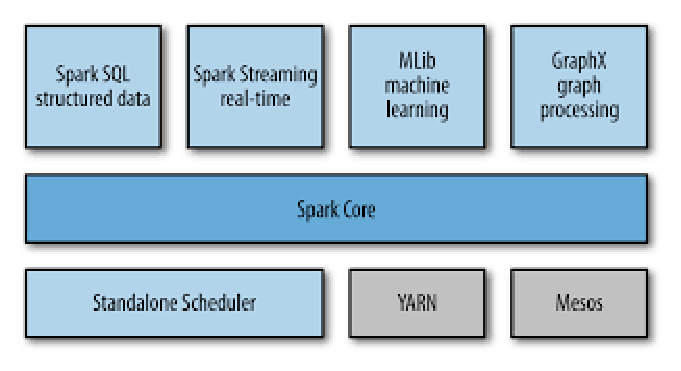
\includegraphics[width=8cm]{1.eps}
	\caption{Architecture of Apache Spark.}\label{fig:ArchitectureSpark}
\end{figure}
\par The main abstraction in Spark is resilient distributed dataset (RDD), which represents a read-only collection of objects distributed across a set of machines. Users can explicitly cache an RDD in memory across machines and reuse it in multiple MapReduce-like parallel operations. RDDs achieve fault tolerance through a notion of lineage: if a partition of an RDD is lost, the RDD has enough information about how it was derived from other RDDs to be able to rebuild just that partition. Although RDDs are not a general shared memory abstraction, they represent a sweet-spot between expressivity on the one hand and scalability and reliability on the other hand, and we have found them wellsuited for a variety of applications. 

\par Now we will show a typical deployment model of spark clusters (Standalone mode); A Spark cluster typically has multiple processes, each running in its own JVM, and a Spark cluster has a master node and multiple worker nodes, which are equivalent to Hadoop's master and slave nodes. The master node has a master daemon process, which manages all the worker nodes. The master daemon allocates resources across applications. The worker node has a worker daemon process, which is responsible for communicating with the master node and managing local executors. The worker also monitors the liveness and resource consumption of the executors. Each application has one driver and multiple executors. The tasks within the same executor belong to the same application. The driver is the process running the main function of the application and creating the SparkContext.
\par The following Figure \ref{fig:RunningSpark} describes the most significant processes.
\begin{figure}
	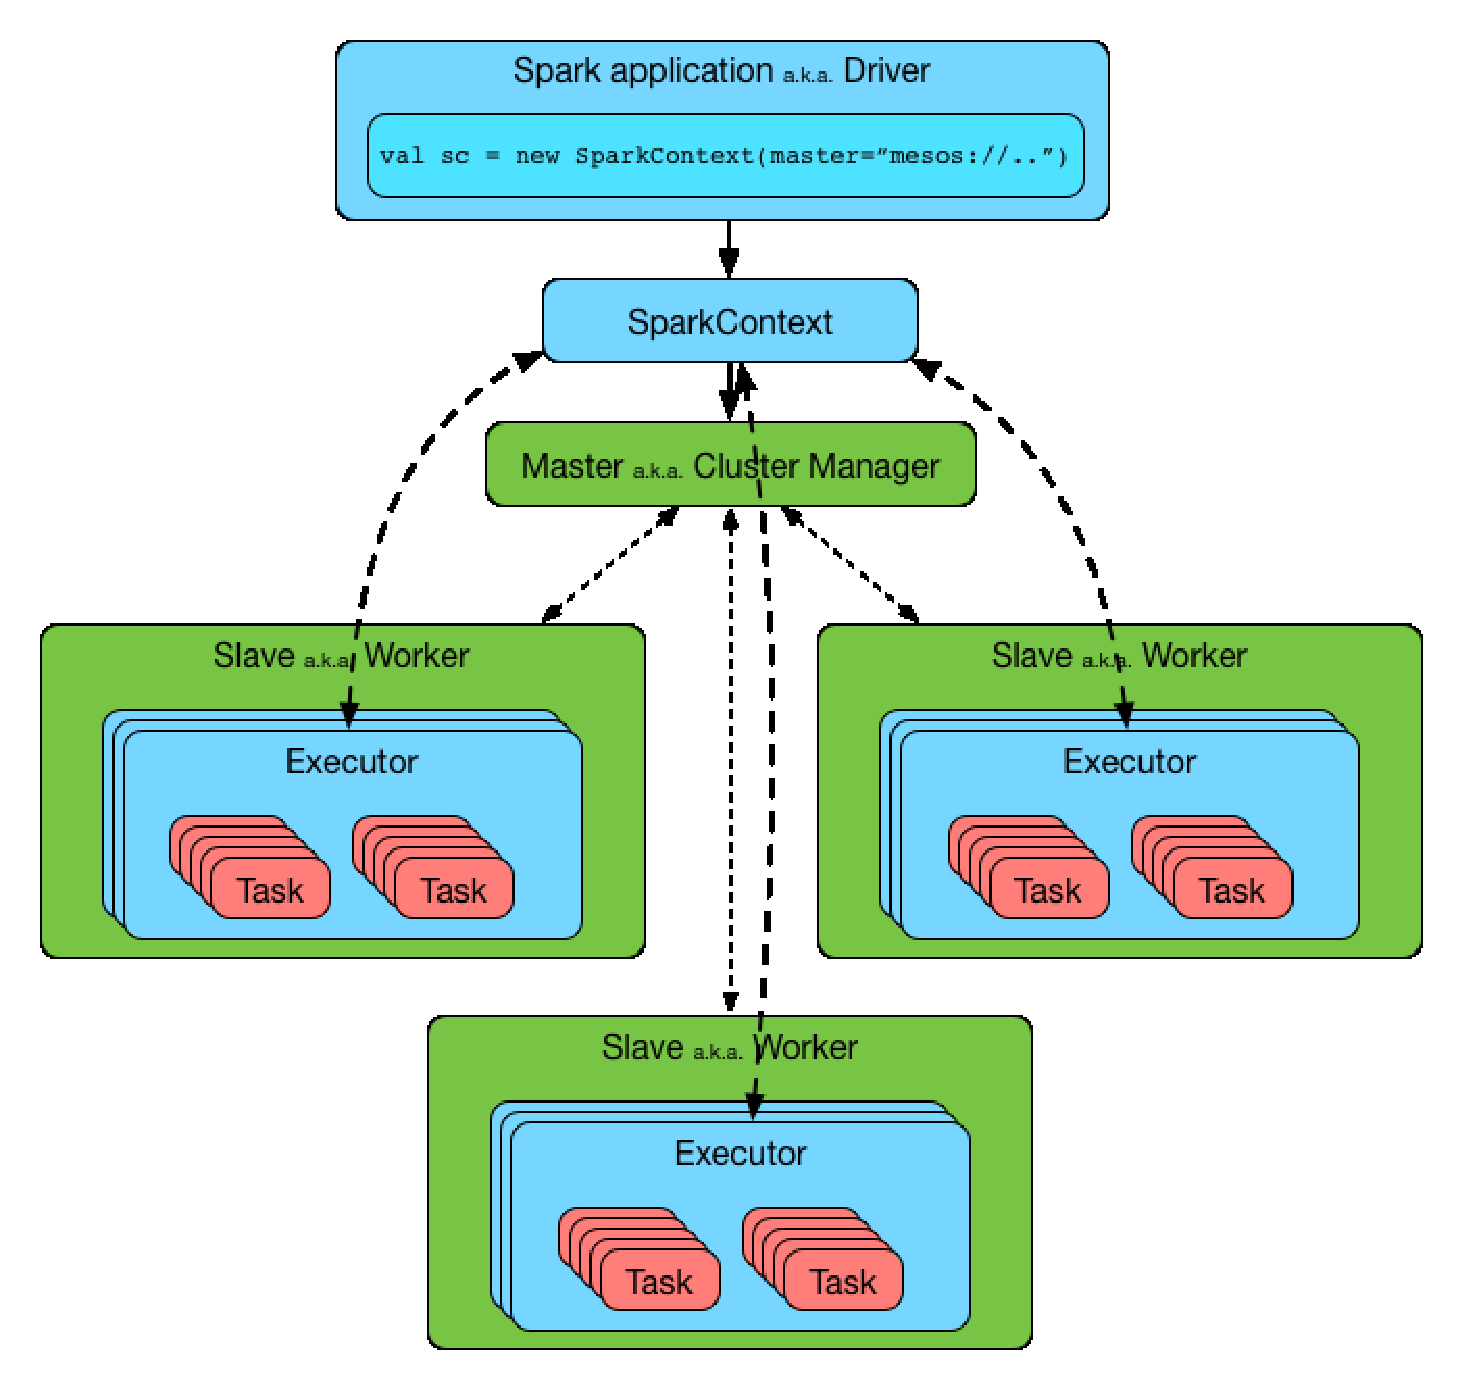
\includegraphics[width=8cm]{4.eps}
	\caption{Running Processes of Spark}\label{fig:RunningSpark}
\end{figure}

\par Because of the in-memory nature of most Spark computations, Spark programs can be bottlenecked by any resource in the cluster: CPU, network bandwidth, or memory. Most often, if the data fits in memory, the bottleneck is network bandwidth, but sometimes, you also need to do some tuning, such as storing RDDs in serialized form, to decrease memory usage. 

\par Fianlly we observe that Apache Spark tunning configuration is very complex, running process is very flexible by users different setting. Moreover we can also sample the parameters by system internal insight. Next we will look at the design of the Hummingbird.


\section{Our Proposed Approach}\label{sec:approach}
\par In this section, a novel approach of adaptively the Spark configurations platform is proposed. And based on the optimizition theroy, we explored a novel algorithm for configuration parameter tuning. And then the specific details of parameter selection, coding method, evaluation function, weighted allocation and Construct the learning examplar are described. 

\par In our problem, the ultimate objective is to find the best configuration. Therefore, the approach does not have enough information to be an accruate performance predictor, but this information is sufficient to find a good configuration within a few steps. As a well known, a greedy algorithm is an algorithmic paradigm that follows the problem solving heuristic of making the locally optimal choice at each stage \cite{greedy} with the hope of finding a global optimum. In many problems, a greedy strategy does not in general produce an optimal solution, but nonetheless a greedy heuristic may yield locally optimal solutions that approximate a global optimal solution in a reasonable time. For example: Particle Swarm Optimization Algorithm(PSO), Ant Colony Optimization Algorithms(ACO), Simulated Annealing Algorithm(SA) etc.  PSO is very popular of all, it has a good convergence of the sequence of solutions. However PSO will always get a local optimalization. This means that determining convergence capabilities of different PSO algorithms and parameters therefore still depends on empirical results. So we will attempt at addressing this issue is the development of an "orthogonal learning" strategy for an improved use of the information already existing in the relationship between p and g, so as to form a leading converging exemplar and to be effective with any PSO topology. The aims are to improve the performance of PSO overall, including faster global convergence, higher solution quality, and stronger robustness \cite{PSO2011}.
\par In this paper, we explore to select some key parameters of Spark configureation which will speed up its performance, and compose them to different setting soluations as the particle positions based on PSO algorithm.  We will also introduce orthogonal learning strategy for improving the PSO performance. Furthermore we will get the global optimalization and improve the performance of Spark.
\par The flowchart of our proposed approach is shown in Fig. \ref{fig:flowchart}.
\begin{figure}\center
	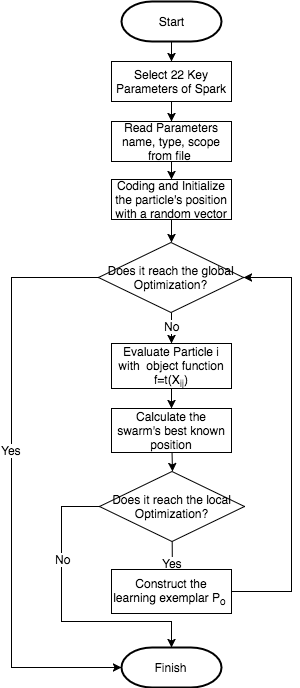
\includegraphics[width=8cm]{flowchart.png}
	\caption{The flowchart of our proposed approach.}\label{fig:flowchart}
\end{figure}
\par From Figure \ref{fig:flowchart}, our approach is described as the following five steps. These parameters are discussed in Section \ref{subsec:parameters}. A coding method of particle positions is presented in Section \ref{subsec:coding}. A object function $f_x$ for evaluation will be proposed in Section \ref{subsec:evaluation}. The weight factors are given in Section \ref{subsec:weight}. Finally, the construction work of learning examplar will detail in Section \ref{subsec:construct}.
\subsection{Parameters Selection}\label{subsec:parameters}
\par In this work, we will select some key parameters from hundreds of Spark parameters \cite{apachesparktuning}. Specially, we investigate the JVM heap, which is key components of Spark \cite{apachesparkmonitoring}. We can see it from Firgure \ref{fig:ParametersJVM} as follows.
\begin{figure}
	\centering
	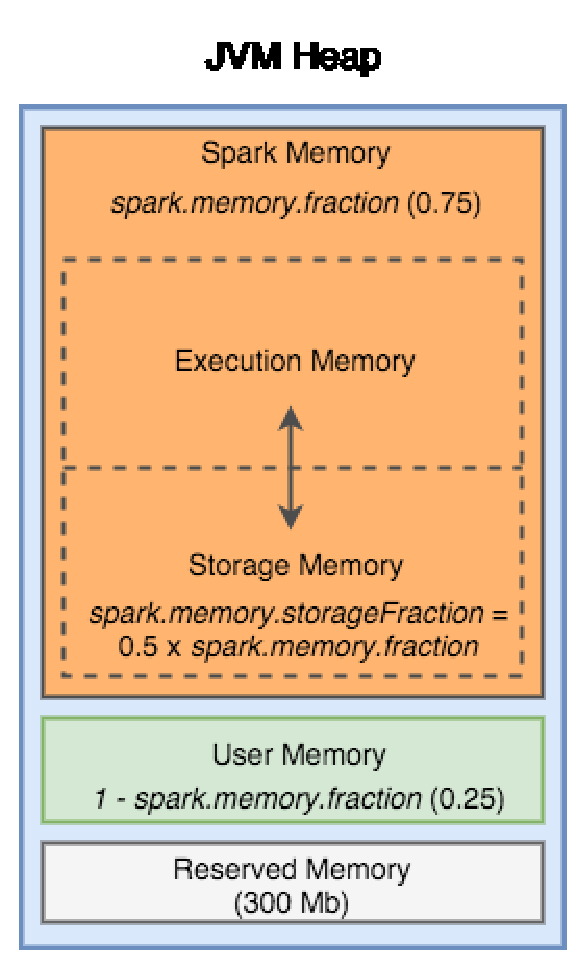
\includegraphics[height=10cm]{3.eps}
	\caption{Parameters of JVM Heap}\label{fig:ParametersJVM}
\end{figure}
 \par Finally, twenty-two parameters are selected, which are shown in Table~\ref{tab:parameters} of Appendix Section.  In Table~\ref{tab:parameters}, the ‘Default’ column lists the default value of each parameter. The 'Meaning' column  explains the meaning of this parameter. The ‘rules of thumb’ column lists the values of each parameter that the industry recommends \cite{SparkConfiguration} \cite{Sparkhub}, and the 'Importance' column is brief introduce the reasons of selection.  The principle for selecting these parameters are listed as follows. 
\begin{itemize}
\item The influences of these parameters cover almost all of the available resources in a cluster, such as CPU, Memory, and Disk.
\item these parameters have a great impact on different modules of Spark, such as schedule, shuffle and compress modules. 
\item these parameters have impact in different levels of a cluster, such as machine-level, cluster-level.
\end{itemize} 
 \par  Generally speaking, various factors that affect the performance of the cluster are comprehensively considered. Based on our testing expertise, these parameters that have significant impact on the performance of Spark are selected.

\par However, parameters selection in a Hummingbird approach is a non-trivial research issue, which can’t only depend on the deep insight of system. we will make up on this in the future work.

\subsection{Coding Method}\label{subsec:coding}
\par Type of Spark parameters have some difference type, such as: Float, Interger, Enumeration, Boolean. Because binary coding will occur the mapping errors when it discretize in the continuous function, in this paper we will adopt the floating coding method. The length of coding is decided by num of parameters. We assume a set of parameters as  $A={p_1, p_2, \cdots,  p_N}$, the value of floating coding will be as $V={v_1, v_2, \cdots , v_N}$. It is shown in Table~\ref{tab:coding}  as follows.

\begin{table}[!htbp]
\caption{Coding of Floating Number} \label{tab:coding} 
\begin{center}
    \begin{tabular}{l*{5}{c}r}
    \hline
    Floating Number & $a_1$ & $a_2$ & $a_3$ & $\cdots$ & $a_N$ \\
    \hline
    Coding & $v_1$ & $v_2$ & $v_3$ & $\cdots$ & $v_N$  \\
    \hline
    \end{tabular}
\end{center}
\end{table}
\par Other types of parameters values also need to convert to floating type.  We assume the range of integer and floating values of parameter  are  $(R^{min}, R^{max}) $, and the range of enumeration is $(R_1, R_2, \cdots, R_N)$. Therefore we will get the normalization formula as follows:
\begin{equation} 
\small
R = \left\{ 
\begin{array}{l l l l}
\frac{R-  R^{min} }{ R^{max}-R^{min} } & Float \\
\frac{R-  R^{min} }{ R^{max}-R^{min} }  & Interger \\
R= true?1.0 : 0.0 & Boolean \\
\frac{i}{N} & Enumeration, R= R_i  
\end{array} \right.
\end{equation}
\par We now deduce the anti-normalization formula as follows.
\begin{equation}
\small
R = \left\{ 
\begin{array}{l l l l}
R' \times {(R^{max}-R^{min})} +R^{min} & Float\\
round(R' \times (R^{max}-R^{min}) + R^{min})  & Interger\\
round(R')= 1?true : false & Boolean\\
{R_{round(R' \times N)}} & Enum
\end{array} \right.
\end{equation}
\par Using this coding method will guarantee robustness and completeness of coding, But there are always exist multiple solutions of the coding space. Therefore, It does not satify the uniqueness. In the Hummingbird, we proposed a new method as follows. After a particle movement, the new position is adjusted. The new position is first normalized to obtain the actual attribute value; then the obtained value is normalized. Since the definition domain and the range of the inverse normalization formula are one-to-one correspondence, the solution of the problem space and the location of the coding space are also one-to-one correspondence. Consequently, it will ensure that the floating coding used satisfy  non-redundancy in this paper.
\subsection{Evaluation Function}\label{subsec:evaluation}
\par As we known, The key criterion of evaluating configuration solution is job running time. Therefore, we will choose job running time as the main evaluation function. We assume that the position $X_{ij}$of particle $ \mathit{i} $ obtained after the $j$th iteration, and  the running time of selected configration is $t(X_{ij})$. So the objective function is expressed as $f=t(X_{ij})$.
\subsection{Weighted Allocation}\label{subsec:weight}
\par The particle swarm optimization algorithm always maintains an acceleration in the case of constant inertia, which facilitates global search at the beginning. However, as the number of iterations increasing, the particles should gradually change from global search to local search. Therefore, the inertia weight should be gradual reduced. Paper \cite{shi1999towards} proposed a inertia weight method to handle it. The inertia weight $w$ is designed as a linearly reduced function, and the formula is as follows.
\begin{equation}
w=w_{max}-\frac{w_{max}-w_{min}}{iter_{max}} \times k
\end{equation}
where the $ w_{max} $ stands for the initial weight, the $ w_{min} $ stands for the final weight. The general values are 0.9 and 0.4 respectively. and $ iter_{max} $ and $ k $ are the max iterations and the current iterations. After modified the inertia weight, particle will transit from global searching to local searching. It guarantees that the alogithm wil have the good convergence. The speed and position of particle will formula as follows.
\begin{equation}
\small
V^{k+1}_{ij} = wV^{k}_{ij} + C_1 R_1(pbest_{ij}-X^k_{ij}) + C_2 R_2 (gbest_j-X^k_{ij})
\end{equation}
\begin{equation}
X^{k+1}_{ij} = X^{k}_{ij} + V^{k+1}_{ij}
\end{equation}
\subsection{Construct the Learning Examplar}\label{subsec:construct}
\par The orthogonal experimental design (OED) offers an ability to discover the best combination levels for different factors with a reasonably small number of experimental samples \cite{dc2000design}, \cite{beijing}. We use the OED method to construct a promising learning exemplar. OED is used to discover the best combination of a particle’s best historical position and its neighborhood’s best historical position. The orthogonal experimental factors are the dimensions of the problem and the levels of each dimension (factor) are the two choices of a particle’s best position value and its neighborhood’s best position value on this corresponding dimension.
\par Let $f_m$ denote the experimental result of the $m$th ($1\leq m \leq M$) combination and $S_nq $ denote the effect of the $q$th ($1 \leq q \leq Q$) level in the $n$th ($1 \leq n \leq N$) factor. The calculation of $S_nq$ is to add up all the $f_m$ in which the level is $q$ in the $n$th factor, and then divide the total count of $z_mnq $, as shown in (6) where $z_mnq $ is 1 if the $m$th experimental test is with the $q$th level of the $n$th factor, otherwise, $z_mnq $ is 0. And $P_0$ is the new learning examplar.
\begin{equation}
 S_nq = \frac{\sum_{m=1}\nolimits M f_m \times z_mnq}{\sum_{m=1}\nolimits M z_mnq}
\end{equation}
In this way, the effect of each level on each factor can be calculated and compared. Compare $f(i)$ and $f (j)$ and the level combination of the better solution is used to construct the vector. A method to further
reduce the number of the orthogonal combinations is to divide the dimensions into several disjoint groups and regard each group as a factor. This method also may be good for the problems whose dimensions are not independent of each other.

\par Next we will evaluate the Hummingbird using some popluar benchmarks.





%
\section{Exiperments and Evaluation}\label{sec:evaluation}
%\subsection{Exiperments}
\par  To evaluate the effectiveness of our method, a Spark cluster with 4 nodes (one master node and three slave node) is deployed. The master node has Xeon processor E3-1200 v3 and 128GB memory. All slave nodes were with eight 3.40 GHz In-tel Core i7 and 8GB memory. Each node has also the same software stack: Ubuntu 16.04 LT and Spark 2.2.0 with Hadoop 2.7.3. 
\par We select WordCount and Sort benchmarks respectively. The iterations of algorithm is 100. The population number is 40. In order to get fast running , we set a threshold $T$, which represents difference degree in the between particles.  The value range of $T$ always between 0 and 0.1. If the threshold value is too big,  the particle will not reach the best position. If the threshold value is too small, the particle will enter the local optimization. And we select twenty-two main parameters, which are shown in Table~\ref{tab:parameters}. Our motivation for choosing these benchmarks is as follows. First, these workloads are simple and easy to understand. Secondly, these benchmarks are representative of real Spark applications, with a wide range of applications. Finally, these benchmarks cover different application types, including I/O intensive, CPU intensive, memory-intensive, and iterativeintensive.
\par We adopt the Sort benchmark first, and get some results as follows. 
\begin{figure}[!htbp]
	%\vspace{-3mm}
	\centering
	\subfigure[The optimization solution when T and N take different values.]
	%\label{fig:sortrunning}
	{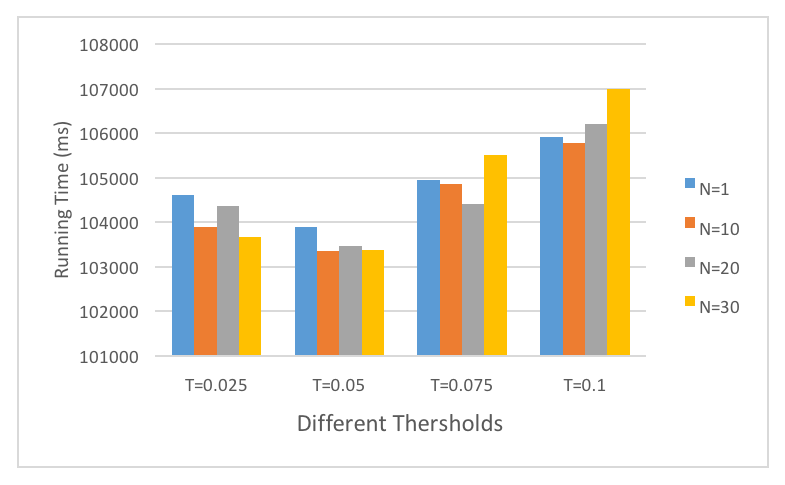
\includegraphics[width=0.48\linewidth]{SortRunningTime.eps}}
	\subfigure[The iterations when T and N take different values.]
	%\label{fig:sortiterations}
	{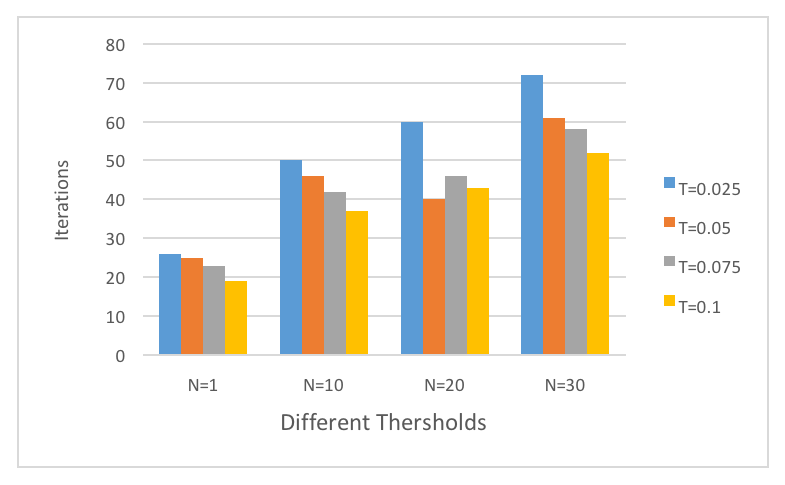
\includegraphics[width=0.48\linewidth]{SortIterations.eps}}\\
	\centering
	\caption{Experiment Results in Sort Benchmark.}
	\vspace{5mm}
	\label{fig:sortcompare}
\end{figure}
\par From above the Figure 6a and Figure 6b, respectively, for $T$ and $N$ take different values, the input 1.6 GB dataset to obtain the optimal solution and algorithm to obtain the optimal solution required for the number of iterations. When $T$ = 0.025 and $N$= 20, the optimal solution is 104,371 ms and the number of iterations is 60. When $T$ = 0.05 and $N$ = 10, the suboptimal solution is 103,360 ms and the number of iterations is 46. In contrast, the optimal solution efficiency is lower by 0.02\%, but the number of iterations is less than 38.68\%. Therefore, when the number of iterations and the optimal solution is taken into account, the algorithm can reach the time of best search status when A = 0.05 and N = 10. 
\par Now we address the Wordcount benchmark. Because the wordcount program has different steps, So we got the following results.
\begin{figure}[!htbp]
	%\vspace{-3mm}
	\centering
	\subfigure[The optimization solution when T and N take different values.]
	%\label{fig:wordcountrunning}
	{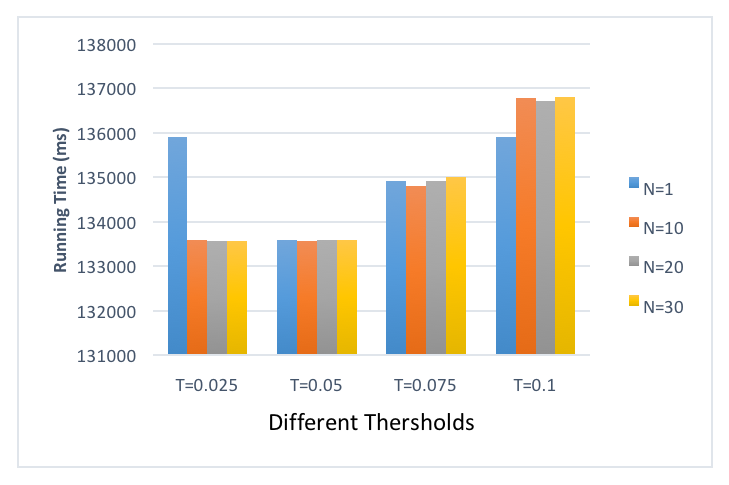
\includegraphics[width=0.48\linewidth]{wordcountRunningTime.eps}}
	\subfigure[The iterations when T and N take different values.]
	%\label{fig:wordcountiterations}
	{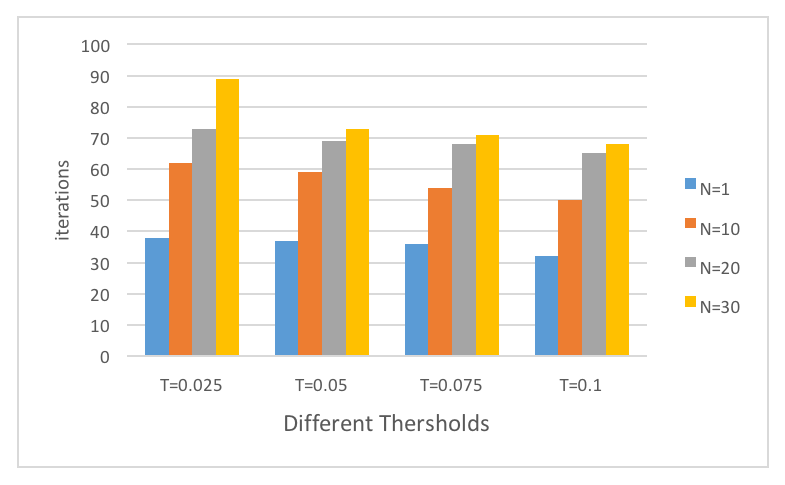
\includegraphics[width=0.48\linewidth]{wordcountIterations.eps}}\\
	\centering
	\caption{Experiment Results in Wordcount Benchmark.}
	\vspace{5mm}
	\label{fig:wordcountcompare}
\end{figure}
\par From above the Figure 7a and Figure 7b, respectively, for $T$ and $N$ take different values, the input 1.6 GB dataset to obtain the optimal solution and algorithm to obtain the optimal solution required for the number of iterations. When $T$ = 0.025 and $N$= 30, the optimal solution is 133,583 ms and the number of iterations is 73. When $T$ = 0.05 and $N$ = 10, the suboptimal solution is 133,560 ms and the number of iterations is 59. In contrast, the optimal solution efficiency is lower by 0.018\%, but the number of iterations is less than 36.63\%. Therefore, when the number of iterations and the optimal solution is taken into account, the algorithm can reach the time of best search status when A = 0.05 and N = 30.
%\begin{figure}
%   \centering
%  \begin{subfigure}[b]{0.5\textwidth}
%        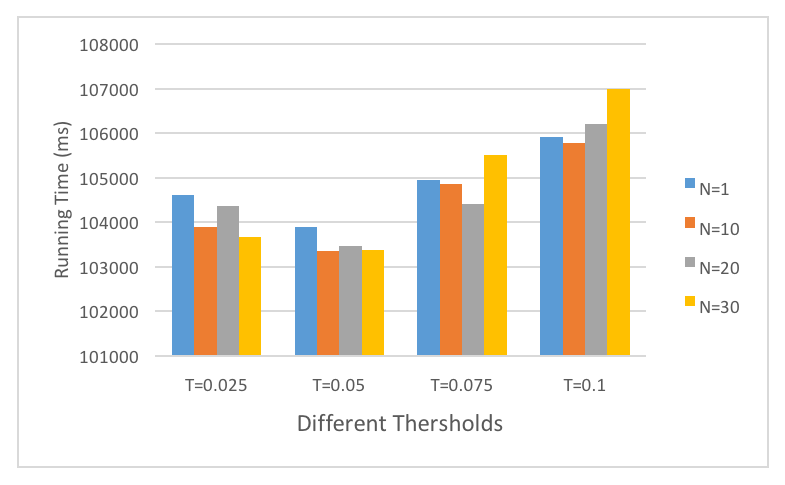
\includegraphics[width=\textwidth]{SortRunningTime.eps}
%        \caption{The optimization solution when T and N take different values}
%        \label{fig:gull}
%    \end{subfigure}
    ~ %add desired spacing between images, e. g. ~, \quad, \qquad, \hfill etc. 
      %(or a blank line to force the subfigure onto a new line)
%    \begin{subfigure}[b]{0.5\textwidth}
%        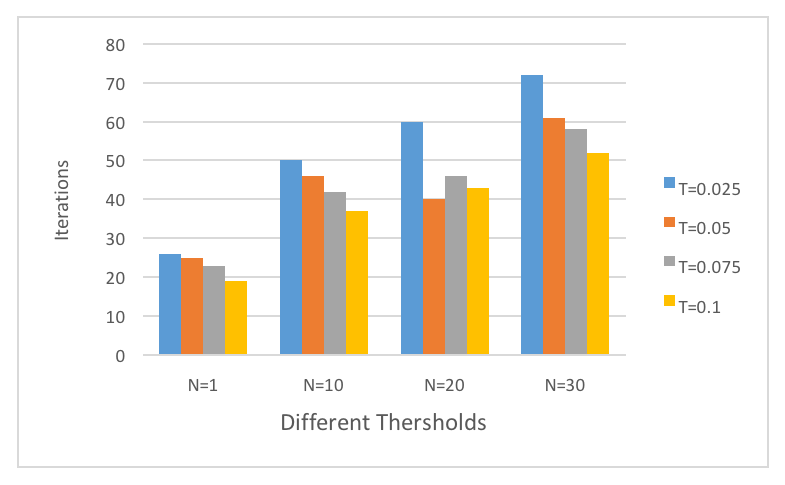
\includegraphics[width=\textwidth]{SortIterations.eps}
%        \caption{The iterations when T and N take different values}
%        \label{fig:tiger}
%    \end{subfigure}
    ~ %add desired spacing between images, e. g. ~, \quad, \qquad, \hfill etc. 
    %(or a blank line to force the subfigure onto a new line)
%    \caption{Experiments in Sort Benchmark}\label{fig:sortcompare}
%\end{figure}

\par Table \ref{tab:runningtimecompare} for the selection of the same size of 20 different input data experiments, respectively, in the default configuration and our proposed approach to find the optimal configuration run under the average running time. It can be seen that compared with the default configuration scheme, the configuration efficiency of the system can be greatly improved by the our proposed approach, and the operation efficiency is more obvious when the input data of job is larger. 
\begin{table}[!htbp]
\centering
\caption{Running Time of Job between Defalut and Optimization.} \label{tab:runningtimecompare} 
\begin{center}
    \begin{tabular}{l*{2}{c}r}
    \hline
    Configuration & Job Size=0.8GB & Job Size =1.6GB & Efficiency(\%) \\
    \hline
    Defalut & 10,675ms & 21,873ms & 28.6 \\
    Optimization & 7,952ms & 14,626ms & 18.9  \\
    \hline
    \end{tabular}
\end{center}
\end{table}

\par   In the other words, we can say our proposed approach is very suit for big data analysis system. Such as Spark platform. It has a good robustness and stability.

\section{conclusion}\label{sec:conclusion}
\par In this paper, Hummingbird: a novel approach of finding optimal configurations for big data analytics is proposed, and Hummingbird  based on PSO  is established.  Experimental results show that Hummingbird has good accuracy and computational performance across diverse workloads for Wordcount and Sort. And experimental results also show that Hummingbird is effective and available to tune the configuration parameters of Spark platform. An average of 28\% performance improvement can be got with the proposed method. Moreover, with the increase of input data, the effect of performance improvement is more obvious.
\par At the same time, the proposed approach is more robust and flexible as it is easier to adapt to changes. Experimental results demonstrate that it is possible to build an effective performance for big data analytics system in a black box manner, that is, in manner of only using observations from the system and without getting its internals.
\par In the future, we will conduct further research on parameters selection in order to select more suitable parameters. And, we will also consider more parameters affecting on the performance,  try to cover all of spark parameters.


% \section{Introduction}
% % no \IEEEPARstart
% This demo file is intended to serve as a ``starter file''
% for IEEE conference papers produced under \LaTeX\ using
% IEEEtran.cls version 1.8b and later.
% % You must have at least 2 lines in the paragraph with the drop letter
% % (should never be an issue)
% I wish you the best of success.
% 
% \hfill mds
%  
% \hfill August 26, 2015
% 
% \subsection{Subsection Heading Here}
% Subsection text here.
% 
% 
% \subsubsection{Subsubsection Heading Here}
% Subsubsection text here.



% An example of a floating figure using the graphicx package.
% Note that \label must occur AFTER (or within) \caption.
% For figures, \caption should occur after the \includegraphics.
% Note that IEEEtran v1.7 and later has special internal code that
% is designed to preserve the operation of \label within \caption
% even when the captionsoff option is in effect. However, because
% of issues like this, it may be the safest practice to put all your
% \label just after \caption rather than within \caption{}.
%
% Reminder: the "draftcls" or "draftclsnofoot", not "draft", class
% option should be used if it is desired that the figures are to be
% displayed while in draft mode.
%
%\begin{figure}[!t]
%\centering
%\includegraphics[width=2.5in]{myfigure}
% where an .eps filename suffix will be assumed under latex, 
% and a .pdf suffix will be assumed for pdflatex; or what has been declared
% via \DeclareGraphicsExtensions.
%\caption{Simulation results for the network.}
%\label{fig_sim}
%\end{figure}

% Note that the IEEE typically puts floats only at the top, even when this
% results in a large percentage of a column being occupied by floats.


% An example of a double column floating figure using two subfigures.
% (The subfig.sty package must be loaded for this to work.)
% The subfigure \label commands are set within each subfloat command,
% and the \label for the overall figure must come after \caption.
% \hfil is used as a separator to get equal spacing.
% Watch out that the combined width of all the subfigures on a 
% line do not exceed the text width or a line break will occur.
%
%\begin{figure*}[!t]
%\centering
%\subfloat[Case I]{\includegraphics[width=2.5in]{box}%
%\label{fig_first_case}}
%\hfil
%\subfloat[Case II]{\includegraphics[width=2.5in]{box}%
%\label{fig_second_case}}
%\caption{Simulation results for the network.}
%\label{fig_sim}
%\end{figure*}
%
% Note that often IEEE papers with subfigures do not employ subfigure
% captions (using the optional argument to \subfloat[]), but instead will
% reference/describe all of them (a), (b), etc., within the main caption.
% Be aware that for subfig.sty to generate the (a), (b), etc., subfigure
% labels, the optional argument to \subfloat must be present. If a
% subcaption is not desired, just leave its contents blank,
% e.g., \subfloat[].


% An example of a floating table. Note that, for IEEE style tables, the
% \caption command should come BEFORE the table and, given that table
% captions serve much like titles, are usually capitalized except for words
% such as a, an, and, as, at, but, by, for, in, nor, of, on, or, the, to
% and up, which are usually not capitalized unless they are the first or
% last word of the caption. Table text will default to \footnotesize as
% the IEEE normally uses this smaller font for tables.
% The \label must come after \caption as always.
%
%\begin{table}[!t]
%% increase table row spacing, adjust to taste
%\renewcommand{\arraystretch}{1.3}
% if using array.sty, it might be a good idea to tweak the value of
% \extrarowheight as needed to properly center the text within the cells
%\caption{An Example of a Table}
%\label{table_example}
%\centering
%% Some packages, such as MDW tools, offer better commands for making tables
%% than the plain LaTeX2e tabular which is used here.
%\begin{tabular}{|c||c|}
%\hline
%One & Two\\
%\hline
%Three & Four\\
%\hline
%\end{tabular}
%\end{table}


% Note that the IEEE does not put floats in the very first column
% - or typically anywhere on the first page for that matter. Also,
% in-text middle ("here") positioning is typically not used, but it
% is allowed and encouraged for Computer Society conferences (but
% not Computer Society journals). Most IEEE journals/conferences use
% top floats exclusively. 
% Note that, LaTeX2e, unlike IEEE journals/conferences, places
% footnotes above bottom floats. This can be corrected via the
% \fnbelowfloat command of the stfloats package.




% \section{Conclusion}
% The conclusion goes here.




% conference papers do not normally have an appendix


% use section* for acknowledgment
 %\section*{Acknowledgment}





% references section

% can use a bibliography generated by BibTeX as a .bbl file
% BibTeX documentation can be easily obtained at:
% http://mirror.ctan.org/biblio/bibtex/contrib/doc/
% The IEEEtran BibTeX style support page is at:
% http://www.michaelshell.org/tex/ieeetran/bibtex/
%\bibliographystyle{IEEEtran}
% argument is your BibTeX string definitions and bibliography database(s)
%\bibliography{IEEEabrv,../bib/paper}
%
% <OR> manually copy in the resultant .bbl file
% set second argument of \begin to the number of references
% (used to reserve space for the reference number labels box)

\bibliographystyle{IEEEtran}
\bibliography{./references}
\section{Appendix}\label{sec:appendix}

\begin{table*}[!htbp]
\caption{Selected Parameters In the Hummingbird} \footnotesize \label{tab:parameters} 
\begin{center}
    \begin{tabular}{ | c | c  | p{4cm} | c | p{5cm} |}
    \hline
    Parameter Name & Default & Meaning & Rules of Thumb & Importance\\ 
    \hline
    spark.driver.memory & 512m & Amount of memory to use for the driver process. & 1g-4g & Directly affect computing performace of spark memory.\\ 
    \hline
    spark.driver.maxResultSize & 1g & Each Spark action in the total size of the serialization results for all partitions. & 1g-8g & It represents a fixed memory overhead per reduce task.\\ 
    \hline
    spark.executor.memory &  1g &Amount of memory to use per executor process.   & 2g-8g & Directly affect computing performace of spark memory.\\
    \hline
     spark.driver.cores & 1 & Number of cores to use for the driver process. & 1-8. & Directly affect the parallelism of the program.\\
    \hline
      spark.executor.cores &  1 & Number of cores to use  per executor process. & 10-40 & Directly affect the parallelism of the program.\\
    \hline
     spark.shuffle.file.buffer &  32k & Size of the in-memory buffer for each shuffle file output stream. & 10-40 & These buffers reduce the number of disk seeks and system calls made in creating intermediate shuffle files.\\
    \hline
     spark.reducer.maxSizeInFlight &  48m & Maximum size of map outputs to fetch simultaneously from each reduce task.  & 24k-96k & This represents a fixed memory overhead per reduce task. \\
    \hline
     spark.shuffle.compress &  true & Whether to compress map output files. & true/false & It will speed up the shuffle action.\\
    \hline
     spark.shuffle.spill.compress &  true & Whether to compress data spilled during shuffles. & true/false & It will speed up the shuffle action.\\
    \hline
     spark.broadcast.compress &  true & Whether to compress broadcast variables before sending them. & true/false & It will speed up the broadcast action.\\
    \hline
     spark.io.compression.codec &  lz4 & The codec used to compress internal data such as RDD partitions, event log, broadcast variables and shuffle outputs. & lz4/lzf/snappy. &  It will speed up all of I/O action.\\
    \hline
     spark.rdd.compress &  false & Whether to compress serialized RDD partitions. & true/fasle & It can save substantial space at the cost of some extra CPU time.\\
    \hline
     spark.default.parallelism &  0.6 & Default number of partitions in RDDs returned by transformations. & 0.4-0.8 & It will add RDD parallelism when user operate join, reduceByKey, and parallelize.\\
    \hline
     spark.memory.fraction &  0.6 & Fraction of (heap space - 300MB) used for execution and storage & 0.4-0.8 & The purpose of this config is to set aside memory for internal metadata, user data structures, and imprecise size estimation in the case of sparse, unusually large records. \\
    \hline
     spark.memory.storageFraction &  0.5  & Amount of storage memory immune to eviction, expressed as a fraction of the size of the region set aside by it. & 0.3-0.8 & The higher this is, the less working memory may be available to execution and tasks may spill to disk more often.\\
       \hline
     spark.broadcast.blockSize &  4m & Size of each piece of a block for TorrentBroadcastFactory. & 2m-8m & It will affect parallelism during broadcast.\\
      \hline
    spark.files.useFetchCache &  true & File fetching will use a local cache that is shared by executors that belong to the same application, which can improve task launching performance when running many executors on the same host. & true/false & This optimization may be disabled in order to use Spark local directories that reside on NFS filesystems.\\    
  \hline
     spark.files.openCostInBytes &  4M & The estimated cost to open a file, measured by the number of bytes could be scanned in the same time. & true/false &the partitions with small files will be faster than partitions with bigger files.\\
  \hline
     spark.storage.memoryMapThreshold &  2m & Size of a block above which Spark memory maps when reading a block from disk. & 1m-4m & It prevents Spark from memory mapping very small blocks.\\
  \hline
    spark.rpc.message.maxSize & true & Maximum message size (in MB) to allow in "control plane" communication. & true/false & It will speed up the network action when  you are running jobs with many thousands of map and reduce tasks.\\
  \hline
    spark.speculation.quantile &  0.75 & Fraction of tasks which must be complete before speculation is enabled for a particular stage. & 0.45-0.9 & It will speed up the task.\\
  \hline
     spark.dynamicAllocation.enabled &  true & Whether to use dynamic resource allocation, which scales the number of executors registered with this application up and down based on the workload. & true/false & It will increase the resource when we are handling a workload .\\
   \hline    
    \end{tabular}
\end{center}	
\end{table*}






 %\begin{thebibliography}{1}
 
 %\bibitem{IEEEhowto:kopka}
 %H.~Kopka and P.~W. Daly, \emph{A Guide to \LaTeX}, 3rd~ed.\hskip 1em %plus
 %  0.5em minus 0.4em\relax Harlow, England: Addison-Wesley, 1999.
 % \end{thebibliography}
 
 % {"isAjaxInProgress_B000AQ24AS":"0","isAjaxComplete_B000AQ24AS":"0"} Thomas H. Cormen (Author) › Visit Amazon's Thomas H. Cormen Page Find All the Books, Re. "Introduction to Algorithms, 3rd Edition (MIT Press) 3rd Edition." Introduction to Algorithms, 3rd Edition (MIT Press): Thomas H. Cormen, Charles E. Leiserson, Ronald L. Rivest, Clifford Stein: 9780262033848: Amazon.com: Books. N.p., n.d. Web. 30 July 2017.

\end{document}


